% --------------------------------------------------------------------------------------------------  %SM: the section read really well and super clear! Really well done JK!
\subsection{Experiment~1: Mechanisms by which turnover influences equilibrium prevalence}
\label{ss:res-prevalence}
Figure~\ref{fig:prevalence} shows the trends in equilibrium STI prevalence among the
high~(\subref{fig:prevalence-high}),
medium~(\subref{fig:prevalence-med}), and
low~(\subref{fig:prevalence-low})
risk groups, at different rates of turnover
which are depicted on the x-axis,
based on duration of time spent in the high risk group.
Figure~\ref{fig:prevalence} reveals an inverted U-shaped relationship
between STI prevalence and turnover in all three risk groups.
That is, equilibrium STI prevalence was higher in systems with slow turnover
versus those with no turnover
(Figure~\ref{fig:prevalence}, region~A).
Equilibrium STI prevalence then peaked at slightly faster turnover
before declining in systems with even faster turnover
(region~B in Figure~\ref{fig:prevalence}).
Comparison of group-specific prevalence in Figure~\ref{fig:prevalence} shows that
the threshold turnover rate at which group-specific prevalence peaked varied by risk group:
prevalence in the high risk group peaked at the lower turnover threshold
(Figure~\ref{fig:prevalence-high}),
while prevalence in low risk group peaked at a higher turnover threshold
(Figure~\ref{fig:prevalence-low}).
To explain the inverted U-shape and different turnover thresholds by group,
we examined the components contributing to prevalence,
first in the high risk group, and then in the low risk group.
\begin{figure}
  % JK: @SM: FYI this horizontal positioning is temporary
  %     I agree it is more intuitive to read vertically as we discussed,
  %     but for now that vertical layout is causing funny LaTeX spacing		%SM: minor detail not worth the effort to revise!....the figure is clear
  \begingroup\centering
  \begin{subfigure}{0.33\linewidth}
    \includegraphics[width=\linewidth]{{1d-prevalence-high-tau=0.1}.pdf}
    \caption{High risk}
    \label{fig:prevalence-high}
  \end{subfigure}%\\
  \begin{subfigure}{0.33\linewidth}
    \includegraphics[width=\linewidth]{{1d-prevalence-med-tau=0.1}.pdf}
    \caption{Medium risk}
    \label{fig:prevalence-med}
  \end{subfigure}%\\
  \begin{subfigure}{0.33\linewidth}
    \includegraphics[width=\linewidth]{{1d-prevalence-low-tau=0.1}.pdf}
    \caption{Low risk}
    \label{fig:prevalence-low}
  \end{subfigure}\\
  \endgroup
  \caption{Relationship between equilibrium STI prevalence
    in high, medium, and low risk groups versus turnover rate.
    Regions A~and~B denote where equilibrium prevalence is increasing and decreasing
    with different rates of turnover, respectively.}
  \label{fig:prevalence}
  \footnotesizeTurnover rate (log scale) is a function of
the duration of time spent in the high risk group $\delta_H$,
where shorter time spent in the high risk group yields faster turnover.
No turnover is indicated by $\delta_H^{-1} = 0.03$,
due to population exit rate $\mu = 0.03$.
\end{figure}
\begin{figure}
  \begingroup\centering
  \begin{subfigure}{0.33\linewidth}
    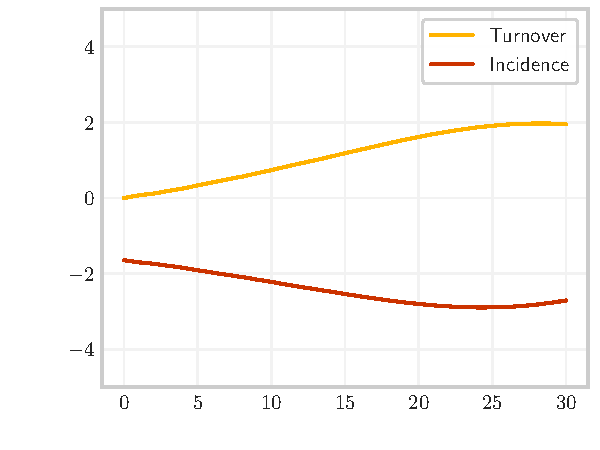
\includegraphics[width=\linewidth]{dX-abs-basic-high-S.pdf}
    \caption{High risk susceptible}
    \label{fig:dX-high-S}
  \end{subfigure}%
  \begin{subfigure}{0.33\linewidth}
    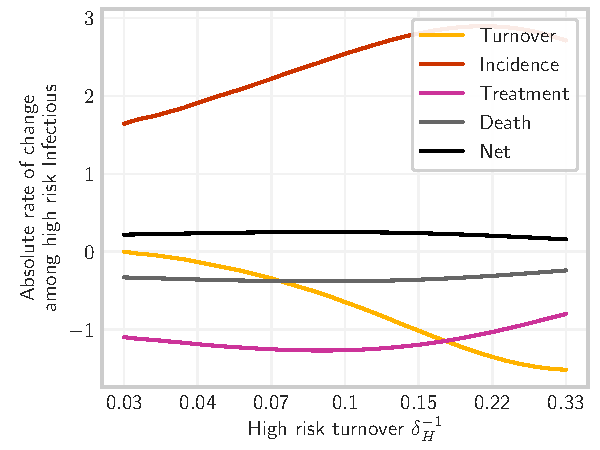
\includegraphics[width=\linewidth]{dX-abs-basic-high-I.pdf}
    \caption{High risk infectious}
    \label{fig:dX-high-I}
  \end{subfigure}%
  \begin{subfigure}{0.33\linewidth}
    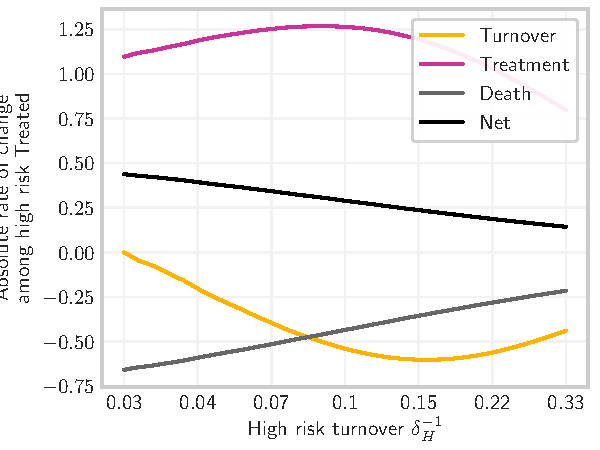
\includegraphics[width=\linewidth]{dX-abs-basic-high-T.pdf}
    \caption{High risk treated}
    \label{fig:dX-high-T}
  \end{subfigure}\\
  \begin{subfigure}{0.33\linewidth}
    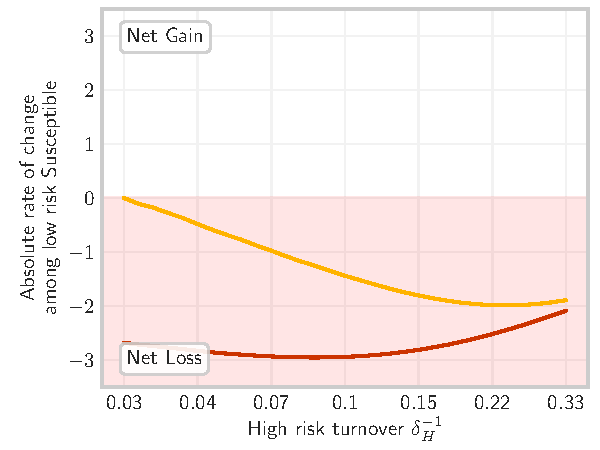
\includegraphics[width=\linewidth]{dX-abs-basic-low-S.pdf}
    \caption{Low risk susceptible}
    \label{fig:dX-low-S}
  \end{subfigure}%
  \begin{subfigure}{0.33\linewidth}
    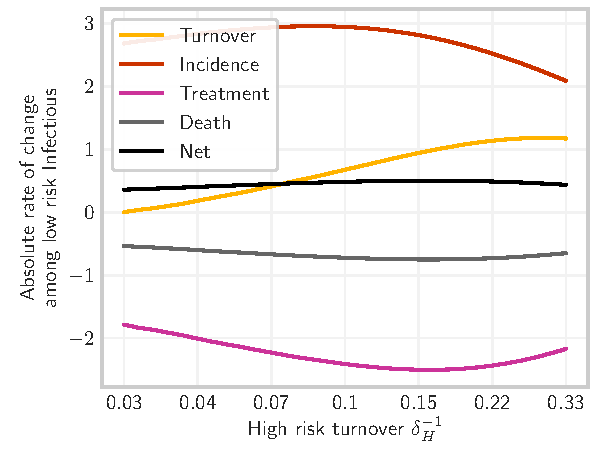
\includegraphics[width=\linewidth]{dX-abs-basic-low-I.pdf}
    \caption{Low risk infectious}
    \label{fig:dX-low-I}
  \end{subfigure}%
  \begin{subfigure}{0.33\linewidth}
    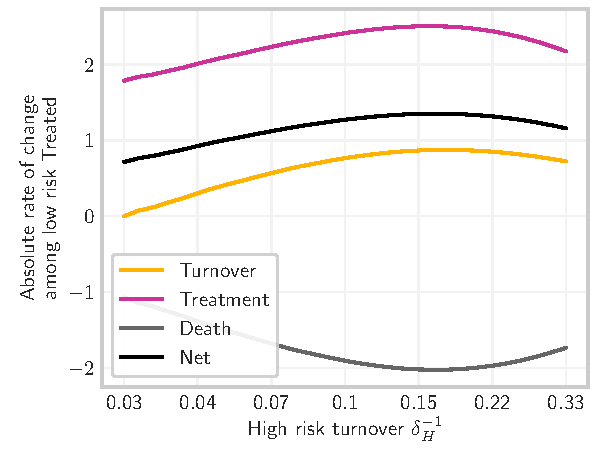
\includegraphics[width=\linewidth]{dX-abs-basic-low-T.pdf}
    \caption{Low risk treated}
    \label{fig:dX-low-T}
  \end{subfigure}\\
  \endgroup
  \caption{Absolute rates of change at equilibrium
    (number of individuals gained/lost per year)
    among individuals in each health state and risk group, due to:
    loss/gain via turnover (yellow), and
    loss/gain via incident infections (red).
    Based on Eq.~(\ref{eq:model}).
    See Figure~\ref{fig:dX-app} for all derivative components.}
  \label{fig:dX}
  \footnotesizeTurnover rate (log scale) is a function of
the duration of time spent in the high risk group $\delta_H$,
where shorter time spent in the high risk group yields faster turnover.
No turnover is indicated by $\delta_H^{-1} = 0.03$,
due to population exit rate $\mu = 0.03$.
\end{figure}
\begin{figure}[!tbp]
  \begingroup\centering
  
\includegraphics[width=0.6\linewidth]{flows-legend-h.pdf}\\
  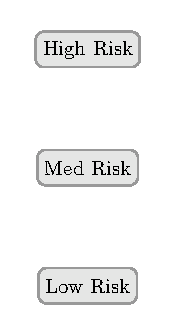
\includegraphics[width=0.11\linewidth]{flows-labels.pdf}
  \begin{subfigure}[t]{0.22\linewidth}
    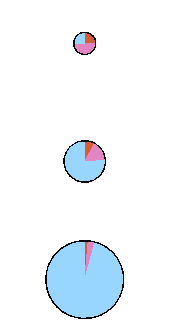
\includegraphics[width=\linewidth]{flows-none.pdf}
    \caption{No turnover}
    \centering\footnotesize $\delta_H^{-1} = 0.062$
    \label{fig:flows-none}
  \end{subfigure}%
  \begin{subfigure}[t]{0.22\linewidth}
    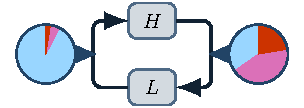
\includegraphics[width=\linewidth]{flows-low.pdf}
    \caption{Slow turnover}
    \centering\footnotesize $\delta_H^{-1} = 0.062$
    \label{fig:flows-low}
  \end{subfigure}%
  \begin{subfigure}[t]{0.22\linewidth}
    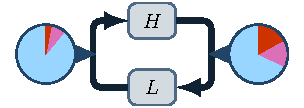
\includegraphics[width=\linewidth]{flows-high.pdf}
    \caption{Fast turnover}
    \centering\footnotesize $\delta_H^{-1} = 0.062$
    \label{fig:flows-high}
  \end{subfigure}%
  \begin{subfigure}[t]{0.22\linewidth}
    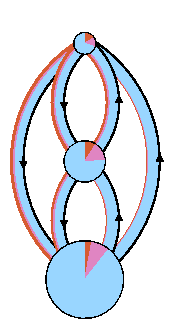
\includegraphics[width=\linewidth]{flows-extr.pdf}
    \caption{Very fast turnover}
    \centering\footnotesize $\delta_H^{-1} = 0.062$
    \label{fig:flows-extr}
  \end{subfigure}\\[0.5em]
  $\null\hspace{0.11\linewidth}
  \underbrace{\hspace{0.44\linewidth}}_{\textrm{Region~A}}
  \underbrace{\hspace{0.44\linewidth}}_{\textrm{Region~B}}$
  \endgroup
  \caption{Depiction of health states of individuals in each risk group
    and of individuals moving between risk groups,
    obtained from models at equilibrium
    under four overall rates of turnover.}
  \footnotesize
  Circle sizes are proportional to risk group sizes.
  Circle slices and arrow widths are also proportional to
  the proportion of health states within risk groups and
  among individuals moving between risk groups, respectively.
  However, circle sizes and arrow widths do not have comparable scales.
  Appendix Figure~\ref{fig:1d-health} illustrates
  proportions of health states versus turnover in full.
  \label{fig:flows}
\end{figure}
\par
Figure~\ref{fig:dX} shows the yearly
gain/loss of individuals via turnover, and
gain/loss via incident infections,
in each health state and risk group,
at equilibrium under different rates of turnover.
Figure~\ref{fig:flows} also illustrates
the distribution of health states in each risk group
and among individuals moving between risk groups
under four different rates of turnover.
% --------------------------------------------------------------------------------------------------
\subsubsection{Influence of turnover on equilibrium prevalence in the high risk group}
\label{sss:res-prev-high}
As shown in Figure~\ref{fig:flows}, at all four rates of turnover
the proportion of individuals who were in the infectious state (STI prevalence)
was largest in the high risk group.
As infectious individuals left the high risk group via turnover,
they were largely replaced by susceptible individuals from lower risk groups
(Figure~\ref{fig:flows-low} and
Figures~\ref{fig:dX-high-S}~vs~\ref{fig:dX-high-I}, yellow).
% SM: for each statement --> give clear example with numbers to support the statement.
% JK: @SM I think maybe this was more needed when Figure dX was not very clear / helpful.
%     I've revised the figure and I think now the examples are not needed
%     and they feel distracting to me on re-read, since there is so much detail here already.
%     What do you think?		SM: agree - the text reads well in reference to the figures and vice versa
%     I leave the content here commented if we want to revive.
% For example, in the context of slow turnover
% ($\delta_H^{-1} = 0.062$),
% infection prevalence in the high risk group was 25\%,
% and the rate of change in the infectious state
% attributable to turnover was
% $\input{\datapath/values/dX/dX-high-I-Turnover-phi=0.062.txt}$ individuals per year
% (Figure~\ref{fig:dX-high-I})
% while the
% rate of change in the susceptible state attributable to turnover was
% $\input{\datapath/values/dX/dX-high-S-Turnover-phi=0.062.txt}$ individuals per year
% (Figure~\ref{fig:dX-high-S}).
The pattern of net outflow of infectious individuals
% JK: FYI changed throughout:  SM: nice!
%     - "removal" & "loss" -> "outflow"
%     - "influx" -> "inflow" for consistency
from the high risk group via turnover
persisted across the range of turnover rates
(Figure~\ref{fig:dX-high-I}, yellow).
This net outflow of infectious individuals via turnover
acted to reduce STI prevalence in the high risk group
% JK: @SM How do you feel about numbering the phenomena like this?
%     I'm not sure, but think it can help a bit		SM: I liked the numbering as I read -- clear and precise and could refer back to where first described
(phenomenon~1).
% JK: originally this was "reduced STI prevalence" (Figure ...)
%     rather than "acted to reduce STI prevalence".
%     I think the distinction is important, as it is only one of the three factors,
%     so we cannot see the effect on prevalence directly without confounding by the other factors,
%     hence, I think it doesn't make sense to reference Figure 4a here yet.
%     Does that make sense? SM: yes, i see your rationale now & agree
Treated individuals were similarly replaced largely by susceptible individuals
(Figure~\ref{fig:flows-low} and
Figures~\ref{fig:dX-high-S}~vs~\ref{fig:dX-high-T}, yellow).
The net replacement of both infectious and treated individuals with susceptible individuals
in the high risk group acted to reduce herd immunity in that group.
% JK: I changed from herd effect to herd immunity throughout
%     since I think the term is more recognizable, and also more specific  
% SM: yes (i tend to like 'effect' in general because 'immunity' makes people think of vaccination, etc. but agree with using immunity here for the reason you bring up - and as the audience for Epidemics will not conflate immunity with vaccination alone, etc)
%     (e.g. I googled "herd effect", and the 1st result was about herd behaviour) SM: LOL
Reduced herd immunity then contributed to a rise in
the number of incident infections in the high risk group,
as the system moved from no turnover to slow turnover
(Figure~\ref{fig:dX-high-I}, red; phenomenon~2).
Incidence was further influenced by a third phenomenon
as systems moved from no turnover to higher rates of turnover:
the net movement of infectious individuals
from high to low risk (Figure~\ref{fig:flows-low})
reduced the average number of partners per year made available by
individuals in the infectious state (Figure~\ref{fig:C-I}).
As shown in Appendix~\ref{aa:eqs-incidence},
modelled incidence in all risk groups was proportional to
the average number of partners per year among infectious individuals
(Figure~\ref{fig:C-I}),
and overall prevalence
(Figure~\ref{fig:prevalence-all}).
Thus, as the average number of partners per year among infectious individuals
fell with faster turnover, incidence decreased
(Figure~\ref{fig:incidence-all}, region~B; phenomenon~3).
\par
Therefore, the inverted U-shaped relationship between turnover rate
and equilibrium STI prevalence in the high risk group was mediated
by the combination of the above three phenomena.
When systems moved from no turnover to slow turnover,
reduction in herd immunity (phenomenon~2) predominated,
leading to increasing equilibrium prevalence with turnover
(Figure~\ref{fig:prevalence-high}, region~A).
When systems were modelled under faster and faster turnover,
outflow of infectious individuals from the group via turnover (phenomenon~1) and
reduction in the average number of partners per year among infectious individuals (phenomenon~3)
% JK: we originally had:
%     "changes in the characteristic of the sexual network
%     (i.e. reduction in average number of partners per year among infectious individuals)"
%     but I find "characteristics of the sexual network" to be a bit vague,	%SM: good point
%     and if we specify what we mean immediately after,
%     I think we might as well skip the first part?		SM: agree. it is more precise and concise now
predominated, leading to lower equilibrium prevalence at faster rates of turnover
(Figure~\ref{fig:prevalence-high}, region~B).
% JK: I removed the sentence below as we say that these experiments aim to explain
%     group-specific prevalence only, not incidence (for more specific focus & scope).
%     The influence on incidence is briefly described in the last sentence of the
%     paragraph just before this one, and I think distracting to circle back to it here
% Accordingly, the inverted U-shaped relationship between turnover rate and equilibrium incidence
% followed a similar pattern within all three groups.
% SM: did not understand the complex sentence below (sentence starting with "Moreover").
%     Not sure how it flowed nor what the main point was. suggest rephrase for clarity
%     (?mutally enforcing exponential decline = wordy and unclear and makes reader feel dumb :)
%     or remove or use suggested edits (but not sure if that is what you meant) = in sentence above.
% JK: We can just remove it.
%     There is a knock-on / snowball / mutually-reinforcing decline in incidence and prevalence:
%     Prevalence among high risk initially declines due to dominance of the 2 factors above,
%     but as a result we have fewer partnerships made available by infectious individuals,
%     so incidence among all groups then declines as a result,
%     which yields fewer infectious individuals, and lower prevalence ...
%     It's kind of circular logic, and not the original driving phenomena
%     so I'm fine to leave it out.  %SM: agree with leaving it out. if raised by reviewers we can bring it up again as a downstream and mutually reinforcing effect...
\begin{figure}
  \begingroup\centering
  \begin{subfigure}[t]{0.33\linewidth}
    \includegraphics[width=\linewidth]{{1d-C-I-tau=0.1}.pdf}
    \caption{Average number of partners per year among infectious individuals}
    \label{fig:C-I}
  \end{subfigure}%
  \begin{subfigure}[t]{0.33\linewidth}
    \includegraphics[width=\linewidth]{{1d-prevalence-all-tau=0.1}.pdf}
    \caption{Overall prevalence}
    \label{fig:prevalence-all}
  \end{subfigure}%
  \begin{subfigure}[t]{0.33\linewidth}
    \includegraphics[width=\linewidth]{{1d-incidence-all-tau=0.1}.pdf}
    \caption{Overall incidence}
    \label{fig:incidence-all}
  \end{subfigure}%
  \\\endgroup
  \caption{Overall incidence and the non-constant factors of incidence versus turnover.
    The product of factors (\subref{fig:C-I}) and (\subref{fig:prevalence-all})
    is proportional to (\subref{fig:incidence-all}) overall incidence.
    See Appendix~\ref{aa:eqs-incidence} for proof.}
  \label{fig:incidence-factors}
  \footnotesizeTurnover rate (log scale) is a function of
the duration of time spent in the high risk group $\delta_H$,
where shorter time spent in the high risk group yields faster turnover.
No turnover is indicated by $\delta_H^{-1} = 0.03$,
due to population exit rate $\mu = 0.03$.
\end{figure}
% --------------------------------------------------------------------------------------------------
\subsubsection{Influence of turnover on equilibrium prevalence in the low risk group}
\label{sss:res-prev-low}
As shown in Figure~\ref{fig:flows}, at equilibrium, the low risk group was
composed mainly of susceptible individuals.
Moving from a system no turnover to one with slow turnover
lead to a net inflow of infectious and treated individuals
(Figures~\ref{fig:dX-low-I}~and~\ref{fig:dX-low-T}, yellow),
and a net removal of susceptible individuals
(Figure~\ref{fig:dX-low-S}, yellow).
% SM: Appendix Figure C.7 currently hides the curves with the legend.
%     Grey and black a bit hard to differentiate; and same with red and pink.
%     might make it harder on the reader.
%     consider using dashed lines to differeniate similar colors, etc.
% JK: I prefer consistent line types, but I increased the color contrast				%SM: agree - see the contrast better now 
%     and popped the legend out in the Appendix version.
The net inflow of infectious individuals
(Figure~\ref{fig:dX-low-I}, yellow) contributed to
% JK: same thing with "led" to vs "contributed to" here
%     re. three factors all contributing to the overall observed pattern					%SM: nice / clear
higher equilibrium prevalence in the low risk group
when the system moved from no turnover to slow turnover
(phenomenon~1).
The inflow of infectious and treated individuals
only slightly reduced the already large proportion who were susceptible
in the low risk group.
Thus, there was little increase in herd immunity within the low risk group
as turnover increased
(phenomenon~2).
However, incident infections still rose in the low risk group
as the system moved from no turnover to slow turnover
(Figure~\ref{fig:dX-low-I}, red)
due to higher incidence in the total population (Figure~\ref{fig:incidence-all})
which was largely driven by
reduced herd immunity in the high risk group
(see Section~\ref{sss:res-prev-high}; phenomenon~2).
Under faster rates of turnover,
incident infections declined in the low risk group
(Figure~\ref{fig:dX-low-I}, red)
due to lower incidence in the total population
(Figure~\ref{fig:incidence-all})
which was driven by
decreasing number of partners per year among infectious individuals
(Figure~\ref{fig:C-I}; phenomenon~3),
as described in Section~\ref{sss:res-prev-high}.
\par
Therefore, as in the high risk group,
the inverted U-shaped relationship between turnover rate
and equilibrium STI prevalence in the low risk group was mediated
by the combination of the above three phenomena.
Moving from no turnover to slow turnover,
the net inflow of infectious individuals (phenomenon~1)
and reduced herd immunity in the high risk group (phenomenon~2)
predominated, leading to higher equilibrium prevalence
(Figure~\ref{fig:prevalence-low}, region~A).
At higher rates of turnover,
a decreasing overall incidence due to
a reduction in the number of partners among infectious individuals (phenomenon~3)
predominated, leading to declining equilibrium prevalence
(Figure~\ref{fig:prevalence-low}, region~B).
\par
In sum, there were three phenomena that
drove shifts in equilibrium STI prevalence across risk groups
at variable rates of turnover:
1)~net flows of infectious individuals from high risk groups into low risk groups;
2)~changes to herd immunity, especially within the high risk group; and
3)~changes to the number of partnerships available with infectious individuals.
% --------------------------------------------------------------------------------------------------
\subsubsection{Influence of turnover on STI prevalence ratio between high and low risk groups}
% JK: I ended up rewriting some of this section, to clarify the logic
%     and remove the part about which peak happened first and comparing the slopes.
As discussed in Sections~\ref{sss:res-prev-high}~and~\ref{sss:res-prev-low},
turnover caused
a net outflow of infectious individuals from the high risk group
(Figure~\ref{fig:dX-high-I}, yellow) and
a net inflow of infectious individuals into the low risk group
(Figure~\ref{fig:dX-low-I}, yellow).
In contrast, the influence of turnover on
the rate of incident infections followed a more similar pattern
in both the high and low risk groups
(Figures~\ref{fig:dX-high-I}~and~\ref{fig:dX-low-I}, red).
Therefore, differences in the influence of turnover on prevalence between risk groups
were driven by net movement of infectious individuals from high to low risk,
causing prevalence in the high and low risk groups
to come closer together with faster turnover.
As shown in Figure~\ref{fig:ratio-prevalence-high-low},
the ratio of equilibrium STI prevalence in the high versus low risk groups
was thus reduced under faster turnover rates.
For example, the prevalence ratio
between high and low risk groups was:
$\input{\datapath/values/turnover-prevalence-ratio-high-low.txt}$
in the model under high turnover ($\delta_H = 5$~years) versus
$\input{\datapath/values/no-turnover-prevalence-ratio-high-low.txt}$
in the model without turnover ($\delta_H = 33$~years)
(Table~\ref{tab:fitting}).
% SM: remove the sentences below....we may get asked to explain by reviewer more
%     --> and if so, then will need to add more or explain this more clearly.
%     I could not easily edit and do not think it adds enough at this stage
%     since the 3 phenomena were already discussed in above sections.
%     And so sentences below feel like they do not flow here.
% JK: Definitely agree about the flow and not adding much.
%     I felt the need to explain since we make the observation in very first results para
%     about the different thresholds, and promise to explain it.
%     So, I think either leave both, or remove both -- what do you think?		SM: below summarized well
Finally, the propensity for equilibrium STI
prevalence to decrease in the high risk group and for
prevalence to increase in the low risk group with faster turnover
-- due to net movement of infectious individuals from high to low risk --		%SM: does the 'due to' refer to both propensities? as it reads, would only refer to the 'prevalence to increase in the low risk group with faster turnover' = what we want yes? suggest parenthesis instead of en-dash then I think?
also explains why prevalence peaked at
slower turnover in the high risk group
(Figure~\ref{fig:prevalence-high}) and
faster turnover in the low risk group
(Figure~\ref{fig:prevalence-low}).
\begin{figure}
  \centerline{\includegraphics[width=0.5\linewidth]{{1d-ratio-prevalence-high-low-tau=0.1}.pdf}}
  \caption{Equilibrium prevalence ratios between high and low risk groups
    under different rates of turnover.}
  \label{fig:ratio-prevalence-high-low}
  \footnotesizeTurnover rate (log scale) is a function of
the duration of time spent in the high risk group $\delta_H$,
where shorter time spent in the high risk group yields faster turnover.
No turnover is indicated by $\delta_H^{-1} = 0.03$,
due to population exit rate $\mu = 0.03$.
\end{figure}
% ==================================================================================================
\subsection{Experiment~2: Inferred risk heterogeneity with versus without turnover}
\label{ss:res-infer}
% SM: moved/edited the text re: predicted prevalance ratios to the above section
%     as I think fits better there right after talking about shrinking prevalence ratios with turnover.
%     In current section, best to go right into fitted results.
% JK: I agree! At first I wasn't sure but I really like it now.
After model fitting,
our two STI transmission models
(one with turnover and one without turnover)
reproduced the target equilibrium STI prevalence values of 20\%,~8.75\%,~3\%,~and~5\%
in the high, medium, low risk groups, and total population, respectively
(Table~\ref{tab:fitting}; Figure~\ref{fig:tpaf-prevalence}).
% JK: re. below: originally read:
%     "had to compensate for the extent to which turnover reduced risk heterogeneity."
%     I reworded and got rid of "risk heterogeneity" since I think that
%     prevalence ratios are more a result of risk heterogeneity than a direct measure of it,  %SM: agree
%     and I would describe model fitting as inference on risk heterogeneity,
%     in which we use the observed prevalence ratios
When fitting the model with turnover to these group-specific prevalence targets,
the fitted numbers of partners per year $C_i$ (the only non-fixed parameter)
had to compensate for the reduction in
STI prevalence ratio between high and low risk groups
(Figure~\ref{fig:ratio-prevalence-high-low}).
As a result, the ratio of fitted partner numbers
between high and low risk groups ($C_H~/~C_L$)
had to be higher in the model with turnover compared to the model without turnover:
$\input{\datapath/values/turnover-[fit]-C-ratio-high-low.txt}$~vs~%
$\input{\datapath/values/no-turnover-[fit]-C-ratio-high-low.txt}$
(Table~\ref{tab:fitting}).
That is, the inferred level of risk heterogeneity was higher
in the model with turnover than in the model without turnover.
\begin{table}
  \caption{Equilibrium partnership formation rates and prevalence
    among the high and low risk groups
    predicted by the models with and without turnover,
    before and after model fitting.}
  \label{tab:fitting}
  \begin{tabularx}{0.7\linewidth}{r *{6}{Y}}
	\toprule
  Model & $C_H$ & $C_L$ & $C_H~/~C_L$ & $P_H$ & $P_L$ & $P_H~/~P_L$\\\midrule
  Base &
    \input{\datapath/fit/Base-C-high.txt}
  & \input{\datapath/fit/Base-C-low.txt}
  & \input{\datapath/fit/Base-C-ratio.txt}
  & \input{\datapath/fit/Base-prevalence-high.txt}
  & \input{\datapath/fit/Base-prevalence-low.txt}
  & \textbf{\input{\datapath/fit/Base-prevalence-ratio.txt}}\\
  V3 &
    \input{\datapath/fit/V3-C-high.txt}
  & \input{\datapath/fit/V3-C-low.txt}
  & \input{\datapath/fit/V3-C-ratio.txt}
  & \input{\datapath/fit/V3-prevalence-high.txt}
  & \input{\datapath/fit/V3-prevalence-low.txt}
  & \textbf{\input{\datapath/fit/V3-prevalence-ratio.txt}}\\
  Base [fit] &
    \input{\datapath/fit/Base-fit-C-high.txt}
  & \input{\datapath/fit/Base-fit-C-low.txt}
  & \textbf{\input{\datapath/fit/Base-fit-C-ratio.txt}}
  & \input{\datapath/fit/Base-fit-prevalence-high.txt}
  & \input{\datapath/fit/Base-fit-prevalence-low.txt}
  & \input{\datapath/fit/Base-fit-prevalence-ratio.txt}\\
  V3 [fit] &
    \input{\datapath/fit/V3-fit-C-high.txt}
  & \input{\datapath/fit/V3-fit-C-low.txt}
  & \textbf{\input{\datapath/fit/V3-fit-C-ratio.txt}}
  & \input{\datapath/fit/V3-fit-prevalence-high.txt}
  & \input{\datapath/fit/V3-fit-prevalence-low.txt}
  & \input{\datapath/fit/V3-fit-prevalence-ratio.txt}\\
  \bottomrule
\end{tabularx}
\end{table}
% ==================================================================================================
\subsection{Experiment~3: Influence of turnover on the tPAF of the high risk group}
\label{ss:res-tpaf}
Finally, we compared the tPAF of the high risk group
projected by the fitted model with turnover and the fitted model without turnover
(Figure~\ref{fig:tpaf-fit}).
The tPAF projected by both models
increased over longer and longer time horizons,
indicating that unmet prevention and treatment needs of the high risk group
were central to epidemic persistence in both fitted models.
The model with turnover projected a larger tPAF at all
time-horizons compared with the tPAF projected by the model without turnover.
The larger tPAF projected by the model with turnover
stemmed from more risk heterogeneity (Table~\ref{tab:fitting})
which led to more onward transmission from the unmet
prevention and treatment needs of the high risk group.
\begin{figure}[!tbp]
  \centerline{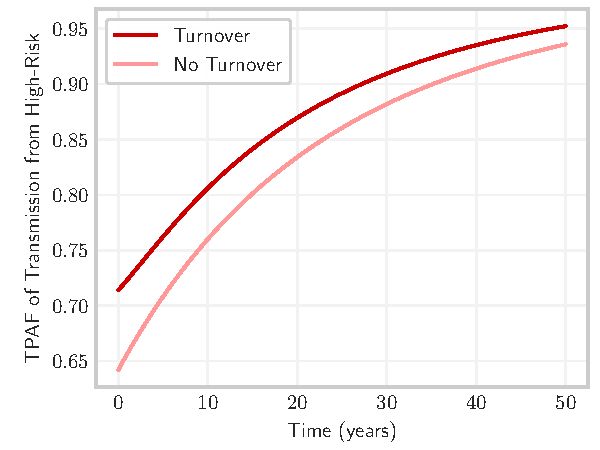
\includegraphics[width=0.5\linewidth]{sit-tpaf-tpaf-high-all-vs=fit.pdf}}
  \caption{Transmission population attributable fraction (tPAF)
    of the high risk group in models with and without turnover,
    after fitting the number of partners per year to group-specific prevalence.}
  \label{fig:tpaf-fit}
\end{figure}